\documentclass{article}
\usepackage{graphicx}

\title{CHAPTER 4}
\author{Murnia Lestari  }
\date{1184006}

\begin{document}

\maketitle

\section{Teori}
\subsection{Fungsi file CSV, Sejarah dan Contoh}
        \begin{enumerate}
            \item Fungsi file CSV
                \paragraph{}Format File .csv digunakan untuk merepresentasikan sebuah data. Format ini termasuk dalam kategori standar file ASCII. Setiap baris dipisahkan dengan enter dan setiap kolom dipisahkan oleh tanda koma atau tanda titik koma. cara membuat file csv , yaitu dengan menggunakan teks editor biasa seperti notepad,sublime,dll. Cara menyimpannya ke dalam ekstensi .csv . File .csv juga dapat dibuat dengan cara mengekspor sebuah file MS Excel atau aplikasi pengolah data lainnya.
            \item Sejarah file CSV
                \paragraph{} CSV atau comma separated value merupakan salah satu tipe file yang digunakan secara luas di dunia programming. Tidak hanya itu CSV  digunakan dalam pengolahan informasi yang dihasilkan spreadsheet untuk diproses lebih lanjut dengan menggunakan mesin analitik. CSV pun dianggap sebagai file yang agnostik karena digunakan oleh berbagai database untuk proses backup data.
            \newpage
            \item Contoh 
               \centerline{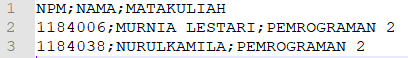
\includegraphics[width=10cm]{figure/0.PNG}} 
        \end{enumerate}
    
    \subsection {Aplikasi-aplikasi yang bisa membuat file CSV}
        \begin{enumerate}
            \item Text Editor (Notepad, Wordpad, dll)
            \item Spreadsheet (Microsoft Excel)
        \end{enumerate}
        
    \subsection{Cara menulis dan membaca file CSV pada Excel}
        \begin{enumerate}
            \item Buka aplikasi excel
            \item K merupakan kolom dan B merupakan baris
            \item Kemudian K1 dan B1 di isi dengan Npm, K1 dan B2 di isi dengan Nama, K1 dan B2 di isi dengan Kelas
            \item Kemudian pada baris ke selanjutnya adalah record.
            \begin{figure}[ht]
                \centerline{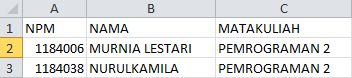
\includegraphics[width=10cm]{figure/1.PNG}}
            \end{figure}
            \item Selanjutnya save as dan pada save as type kita ganti jadi csv (Comman delimited)
            \newpage
            \begin{figure}[ht]
                \centerline{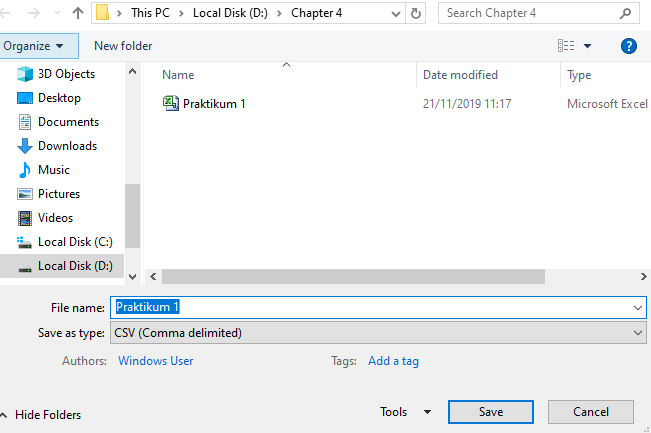
\includegraphics[width=10cm]{figure/2.PNG}}
            \end{figure}
            \item Maka akan file csv telah dibuat.
        \end{enumerate}
    
    \subsection{Sejarah library CSV}
        \paragraph{} Format data yang disebut CSV (Comma Separated Values) adalah format data impor dan ekspor yang paling umum untuk spreadsheet dan basis data. Format CSV digunakan untuk menggambarkan format dengan cara yang standar di RFC 4180 . Kurangnya standar yang didefinisikan dengan baik berarti bahwa perbedaan harus terdapat dalam data yang diproduksi dan dipakai oleh aplikasi yang berbeda.
        
    \subsection{Sejarah library Pandas}
        \paragraph{}merupakan library analisis data yang mempunyai struktur data , library pandas diperlukan untuk mengubah bentuk data bahasa pemrograman menjadi bentuk tabel. 
    
    \subsection{Fungsi-fungsi yang terdpat pada library CSV}
        \begin{enumerate}
            \item Reader
                \paragraph{} Fungsi ini digunakan untuk membaca isi file berformat CSV dari list.
                \newpage\begin{figure}[ht]
                \centerline{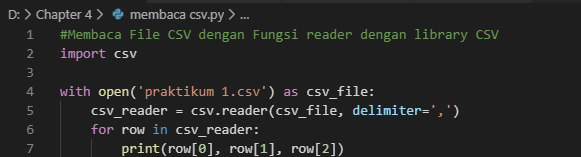
\includegraphics[width=10cm]{figure/3.PNG}}
            \end{figure}
            \item DictReader
                \paragraph{}  Fungsi ini digunakan untuk membaca isi file berformat CSV dari dictionary.
                \begin{figure}[ht]
                \centerline{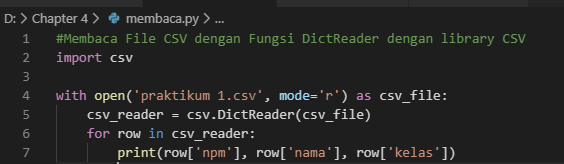
\includegraphics[width=10cm]{figure/4.PNG}}
            \end{figure}
            \item Write
                \paragraph{} Fungsi ini digunakan untuk menulis file berformat CSV dari list.
                 \begin{figure}[ht]
                \centerline{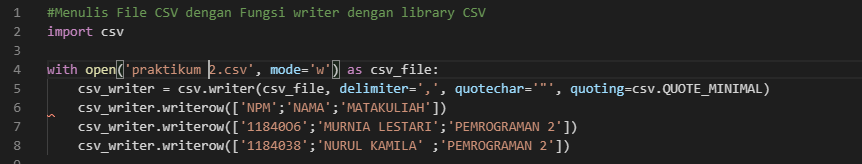
\includegraphics[width=10cm]{figure/5.PNG}}
            \end{figure}
            \newpage\item DictWrite
                \paragraph{}  Fungsi ini digunakan untuk menulis file berformat CSV dari dictionary.
              \begin{figure}[ht]
                \centerline{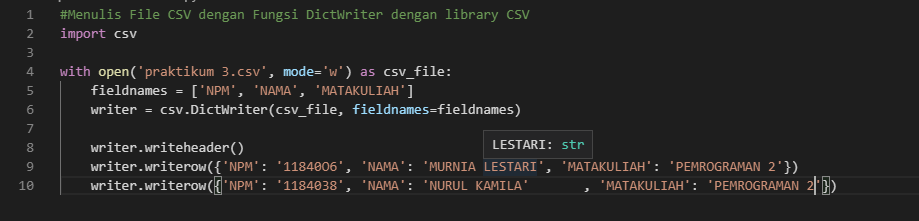
\includegraphics[width=10cm]{figure/6.PNG}}
            \end{figure}
        \end{enumerate}
     
    \subsection{Fungsi-fungsi yang terdpat pada library Pandas}
        \begin{enumerate}
            \item Read\_csv
                \paragraph{} Fungsi ini digunakan untuk membaca isi file berformat CSV.
                \begin{figure}[ht]
                \centerline{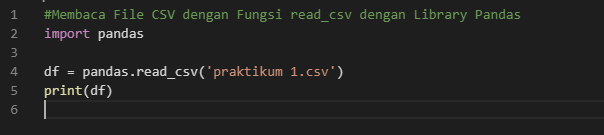
\includegraphics[width=10cm]{figure/7.PNG}}
            \end{figure}
            \item To\_csv
                \paragraph{} Fungsi ini digunakan untuk menulis file berformat CSV.
               \begin{figure}[ht]
                \centerline{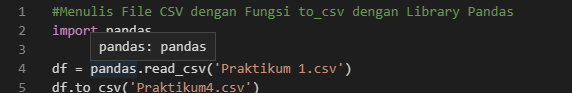
\includegraphics[width=10cm]{figure/8.PNG}}
            \end{figure}
        \end{enumerate}
    
\section{Keterampilan Pemrograman}
    \subsection*{Soal 1}
        \paragraph{}Buatlah fungsi (file terpisah/library dengan nama NPM csv.py) untuk membuka file csv dengan lib csv mode list. Berikut adalah pemanggilan file csv dengan library csv yang menggunakan list.
        \begin{figure}[ht]
                \centerline{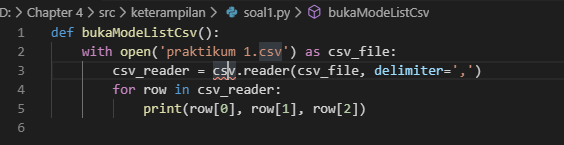
\includegraphics[width=10cm]{figure/a.PNG}}
            \end{figure}
        
    \subsection*{Soal 2}
        \paragraph{}Buatlah fungsi (file terpisah/library dengan nama NPM csv.py) untuk membuka file csv dengan lib csv mode dictionary. Berikut adalah pemanggilan file csv dengan library csv yang menggunakan dictionary.
        \begin{figure}[ht]
                \centerline{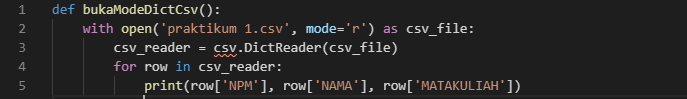
\includegraphics[width=10cm]{figure/b.PNG}}
            \end{figure}
        
    \subsection*{Soal 3}
        \paragraph{}Buatlah fungsi (file terpisah/library dengan nama NPM pandas.py) untuk membuka file csv dengan lib csv mode list.
         \begin{figure}[ht]
                \centerline{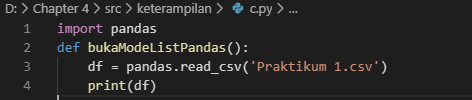
\includegraphics[width=10cm]{figure/c.PNG}}
            \end{figure}
  \newpage      
    \subsection*{Soal 4}
        \paragraph{}Buatlah fungsi (file terpisah/library dengan nama NPM pandas.py) untuk membuka file csv dengan lib csv mode dictionary. 
         \begin{figure}[ht]
                \centerline{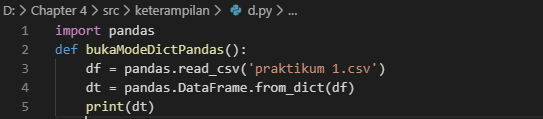
\includegraphics[width=10cm]{figure/d.PNG}}
            \end{figure}
        
    \subsection*{Soal 5}
        \paragraph{}Buatlah fungsi pada file NPMpandas.py, untuk mengubah format tanggal menjadi standar dataframe. 
        \begin{figure}[ht]
                \centerline{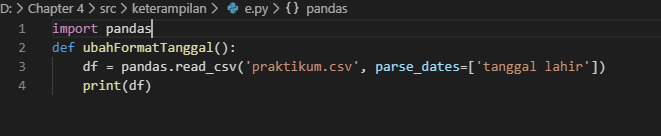
\includegraphics[width=10cm]{figure/e.PNG}}
            \end{figure}
    
    \subsection*{Soal 6}
        \paragraph{}Buatlah fungsi pada file NPMpandas.py, untuk mengubah index kolom. 
        \begin{figure}[ht]
                \centerline{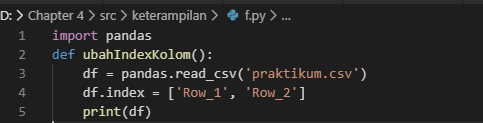
\includegraphics[width=10cm]{figure/f.PNG}}
            \end{figure}
    
    \newpage\subsection*{Soal 7}
        \paragraph{}Buatlah fungsi pada file NPMpandas.py, untuk mengubah atribut atau nama kolom .
        \begin{figure}[ht]
                \centerline{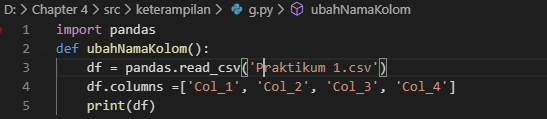
\includegraphics[width=10cm]{figure/g.PNG}}
            \end{figure}
    \subsection*{Soal 8}
        \paragraph{}Buatlah program main.py untuk menggunakan library NPMcsv.py yang dapat membuat file dan membaca file csv.
\begin{figure}[ht]
                \centerline{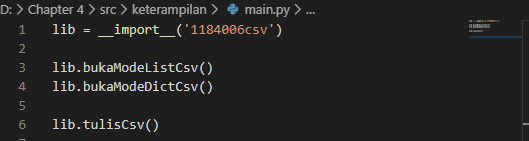
\includegraphics[width=10cm]{figure/i.PNG}}
            \end{figure}
        
    \subsection*{Soal 9}
        \paragraph{}Buatlah program main.py untuk menggunakan library NPMpandas.py yang dapat membuat file dan membaca file csv.
       \begin{figure}[ht]
            \centerline{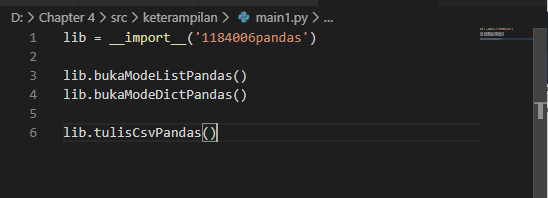
\includegraphics[width=10cm]{figure/j.PNG}}
            \end{figure}
    
\newpage
\section{Penanganan error}
    \paragraph{}Dalam menulis kode program python haruslah berhati-hati karena bahasa pemrograman python sangatlah case sensitive. Penanganan erro yang dapat digunakan adalah dengan try and except
   \begin{figure}[ht]
            \centerline{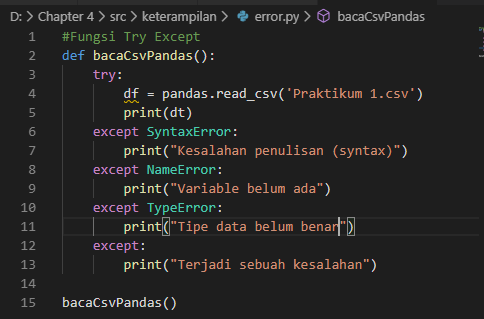
\includegraphics[width=10cm]{figure/k.PNG}}
            \end{figure}
    

  

\end{document}
